\documentclass[11pt]{article}
\usepackage{graphicx}
\usepackage{hyperref}
\usepackage{amsmath}
\usepackage{amsthm}
\usepackage{amssymb}
\usepackage[all=normal,floats,leading,paragraphs,charwidths,tracking,wordspacing]{savetrees}
\usepackage{float}
\usepackage[version = 4]{mhchem}
\usepackage{multirow}
\usepackage{commath}
\usepackage{booktabs}
\usepackage{subcaption}
\renewcommand{\arraystretch}{1.2}
\usepackage{siunitx}
\sisetup{detect-all}
\DeclareSIUnit{\atm}{atm}
\usepackage{listings}
\usepackage{color} %red, green, blue, yellow, cyan, magenta, black, white
\definecolor{mygreen}{RGB}{28,172,0} % color values Red, Green, Blue
\definecolor{mylilas}{RGB}{170,55,241}
\usepackage[a4paper,margin=15mm]{geometry}
\numberwithin{equation}{section}
\setlength{\parskip}{\baselineskip}
\setlength{\parindent}{0pt}
\hypersetup{
    colorlinks=true,
    linkcolor=black,
    filecolor=black,      
    urlcolor=black,
    citecolor=black
}
\urlstyle{same}
\lstset{language=Matlab,%
    %basicstyle=\color{red},
    breaklines=true,%
    morekeywords={matlab2tikz},
    keywordstyle=\color{blue},%
    morekeywords=[2]{1}, keywordstyle=[2]{\color{black}},
    identifierstyle=\color{black},%
    stringstyle=\color{mylilas},
    commentstyle=\color{mygreen},%
    showstringspaces=false,%without this there will be a symbol in the places where there is a space
    numbers=left,%
    numberstyle={\tiny \color{black}},% size of the numbers
    numbersep=9pt, % this defines how far the numbers are from the text
    emph=[1]{for,end,break},emphstyle=[1]\color{red}, %some words to emphasise
    %emph=[2]{word1,word2}, emphstyle=[2]{style},    
}
\begin{document}
\title{\textbf{UCL Mechanical Engineering 2021/2022}\\MECH0024 Thermodynamics Coursework}
\author{RFLH9}
\date{\today}
\maketitle
\tableofcontents
\listoffigures
\listoftables
\newpage
\section{Question 1}
\subsection{Solar power available}
At the time of measurement, the orbital characteristics are as follows.

Solar declination:
\begin{gather}
    \theta_d = \SI{-12}{\degree}
\end{gather}
Polar angle at latitude \SI{51.5}{\degree}:
\begin{gather}
    \theta = 90 - 51.5 = \SI{38.5}{\degree}
\end{gather}
Hour angle at 11am:
\begin{gather}
    \phi = \frac{11\cdot 360}{24} -90 = \SI{75}{\degree}
\end{gather}
Solar azimuth angle:
\begin{gather}
    \cos \psi = \cos \theta_d \sin\theta \sin \phi + \sin\theta_d \cos \theta\\
    \psi = \arccos\left[\cos \left(-12\right)\sin\left(38.5\right)\sin\left(75\right) + \sin\left(-12\right)\cos\left(38.5\right)\right]\\
    \psi = \SI{64.82}{\degree} \textrm{ or}\\
    \cos\psi = 0.43;
\end{gather}
Air mass ratio:
\begin{gather}
    M = \sec\psi\\
    M = 2.35
\end{gather}
Solar flux:
\begin{gather}
    E = 1353\left(0.057+0.83e^{-0.5M}\right) \si{\watt\per\meter\squared}\\
    E = \SI{220.18}{\watt\per\meter\squared}
\end{gather}
The orbital characteristics for when the solar panels are orientated normal to the sun's rays are as follows:
\begin{table}[H]
    \centering
    \begin{tabular}{@{}ll@{}}
        \toprule
        Solar declination, $\theta_d$ & \SI{-5}{\degree}    \\
        Polar angle, $\theta$         & \SI{38.5}{\degree}  \\
        Hour angle, $\phi$            & \SI{90}{\degree}    \\ 
        \bottomrule
    \end{tabular}
    \caption{Orbital characteristics when panels are normal to sun's rays.}
\end{table}
Therefore:
\begin{gather}
    \theta + \theta_d + \alpha = \phi\\
    38.5 - 5 + \alpha = 90\\
    \alpha = \SI{56.5}{\degree}
\end{gather}
Intensity of radiation for collector inclined at $\alpha$ degrees to normal:
\begin{gather}
    E_{\alpha} = E\left[\cos \theta_d \sin\left(\theta + \alpha\right)\sin\phi + \sin\theta_d \cos\left(\theta + \alpha\right)\right]
    E_{\alpha} = \SI{211.23}{\watt\per\square\meter}
\end{gather}
Area of collectors ($A_p$) is \SI{920}{\meter\squared}, therefore intensity of radiation for total collector area is:
\begin{gather}
    \textrm{Incident solar energy} = 211.23\cdot920\cdot10^{-3} = \SI{194.33}{\kilo\watt}
\end{gather}
Looking at the sources of lost energy in our system, we have energy lost due to convection to atmosphere and re-radiated energy. We also have the heat transfer to the working fluid. This must equal the energy in, which is equal to the incident solar energy multiplied by the absorptivity of the collector surface.

Energy absorbed by the collector:
\begin{gather}
    \theta_{solar} = \textrm{incident solar energy} \cdot A
\end{gather}
where $A$ is absorptivity of the collector surface.

Convection to atmosphere:
\begin{gather}
    \theta_{conv} = A_ph\left(T_s - T_a\right)
\end{gather}
where where $A_p$ is area of collector, $h$ is convective heat transfer coefficient between the collector surface and the surrounding air, $T_s$ is average temperature of collector surface, $T_a$ is the temperature of the surrounding air. 

Re-radiated energy:
\begin{gather}
    \theta_{rad} = A_p \varepsilon\sigma\left(T_s^4\right)
\end{gather}
where $\varepsilon$ is emissivity of collector surface, $\sigma$ is Stefan-Boltzmann constant.

The above constants are given in the question. MATLAB was used to calculate the solar power available at the collectors following losses:
\lstinputlisting{mCode/q1.m}
Here we can see that our final answer is stored in the variable \texttt{powerAvail}:
\begin{gather}
    \texttt{powerAvail} = \SI{51.065}{\kilo\watt}
\end{gather}
\subsection{Viability of proposed provision}
We can compare the needs of the developer by using UCL as an example. As one of the largest universities in London, UCL's demand would be similar to the new development. UCL's heating and hot water demand in 2019 is stated to be around 60 million kWh. The proposed solution would easily cover UCL's energy demand (assuming constant power demand ~7000kW) \cite{b1}. The proposed solution would cover peak demands, with spare energy to cover any growth by the developers. This spare energy could be sold on the national grid, reimbursing the developer for the initial cost of the array. 

Since the UK is at a relatively high latitude with mild weather, we may see that our collectors do not operate efficiently for most of the year. During winter months, the ability to collect solar energy may be severely impaired due to frequent inclement weather. By looking at data from UCL regarding the consumption of energy by individual buildings, we see that the primary consumers of heating and domestic water are student accommodation buildings \cite{b2}. Through the utilisation of double-glazing, insulation and smart energy meters, these buildings can be constructed to be more energy efficient as to reduce the overall demand of central heating. These buildings also typically see more use during the evening hours and throughout the night, as students return from class and to rest. One problem that arises is that during these hours, no hot water can be generated. Other technologies such as hot water storage tanks can be used during the night to make up for this. The panels would be able to store the sun's energy from the day and use it during the night period. 

The UK primarily generates its heating via gas boilers, these solar panels would reduce the carbon footprint of the campus greatly. They are also typically mounted on rooftops and hence are non-invasive, not requiring additional space (which may be expensive/destroy wildlife). The recommendation would be to approve such a development as it meets the demand of the client, whilst being cost-effective and reducing the carbon footprint of the campus. 
\section{Question 2}
\subsection{a}
\subsubsection{Irreversibility associated with increase in steady flow exergy of steam}
Assumptions:
\begin{itemize}
    \item Steady flow state.
    \item KE and PE are negligible
    \item Fluid properties are constant.
\end{itemize}
\begin{figure}[H]
    \centering
    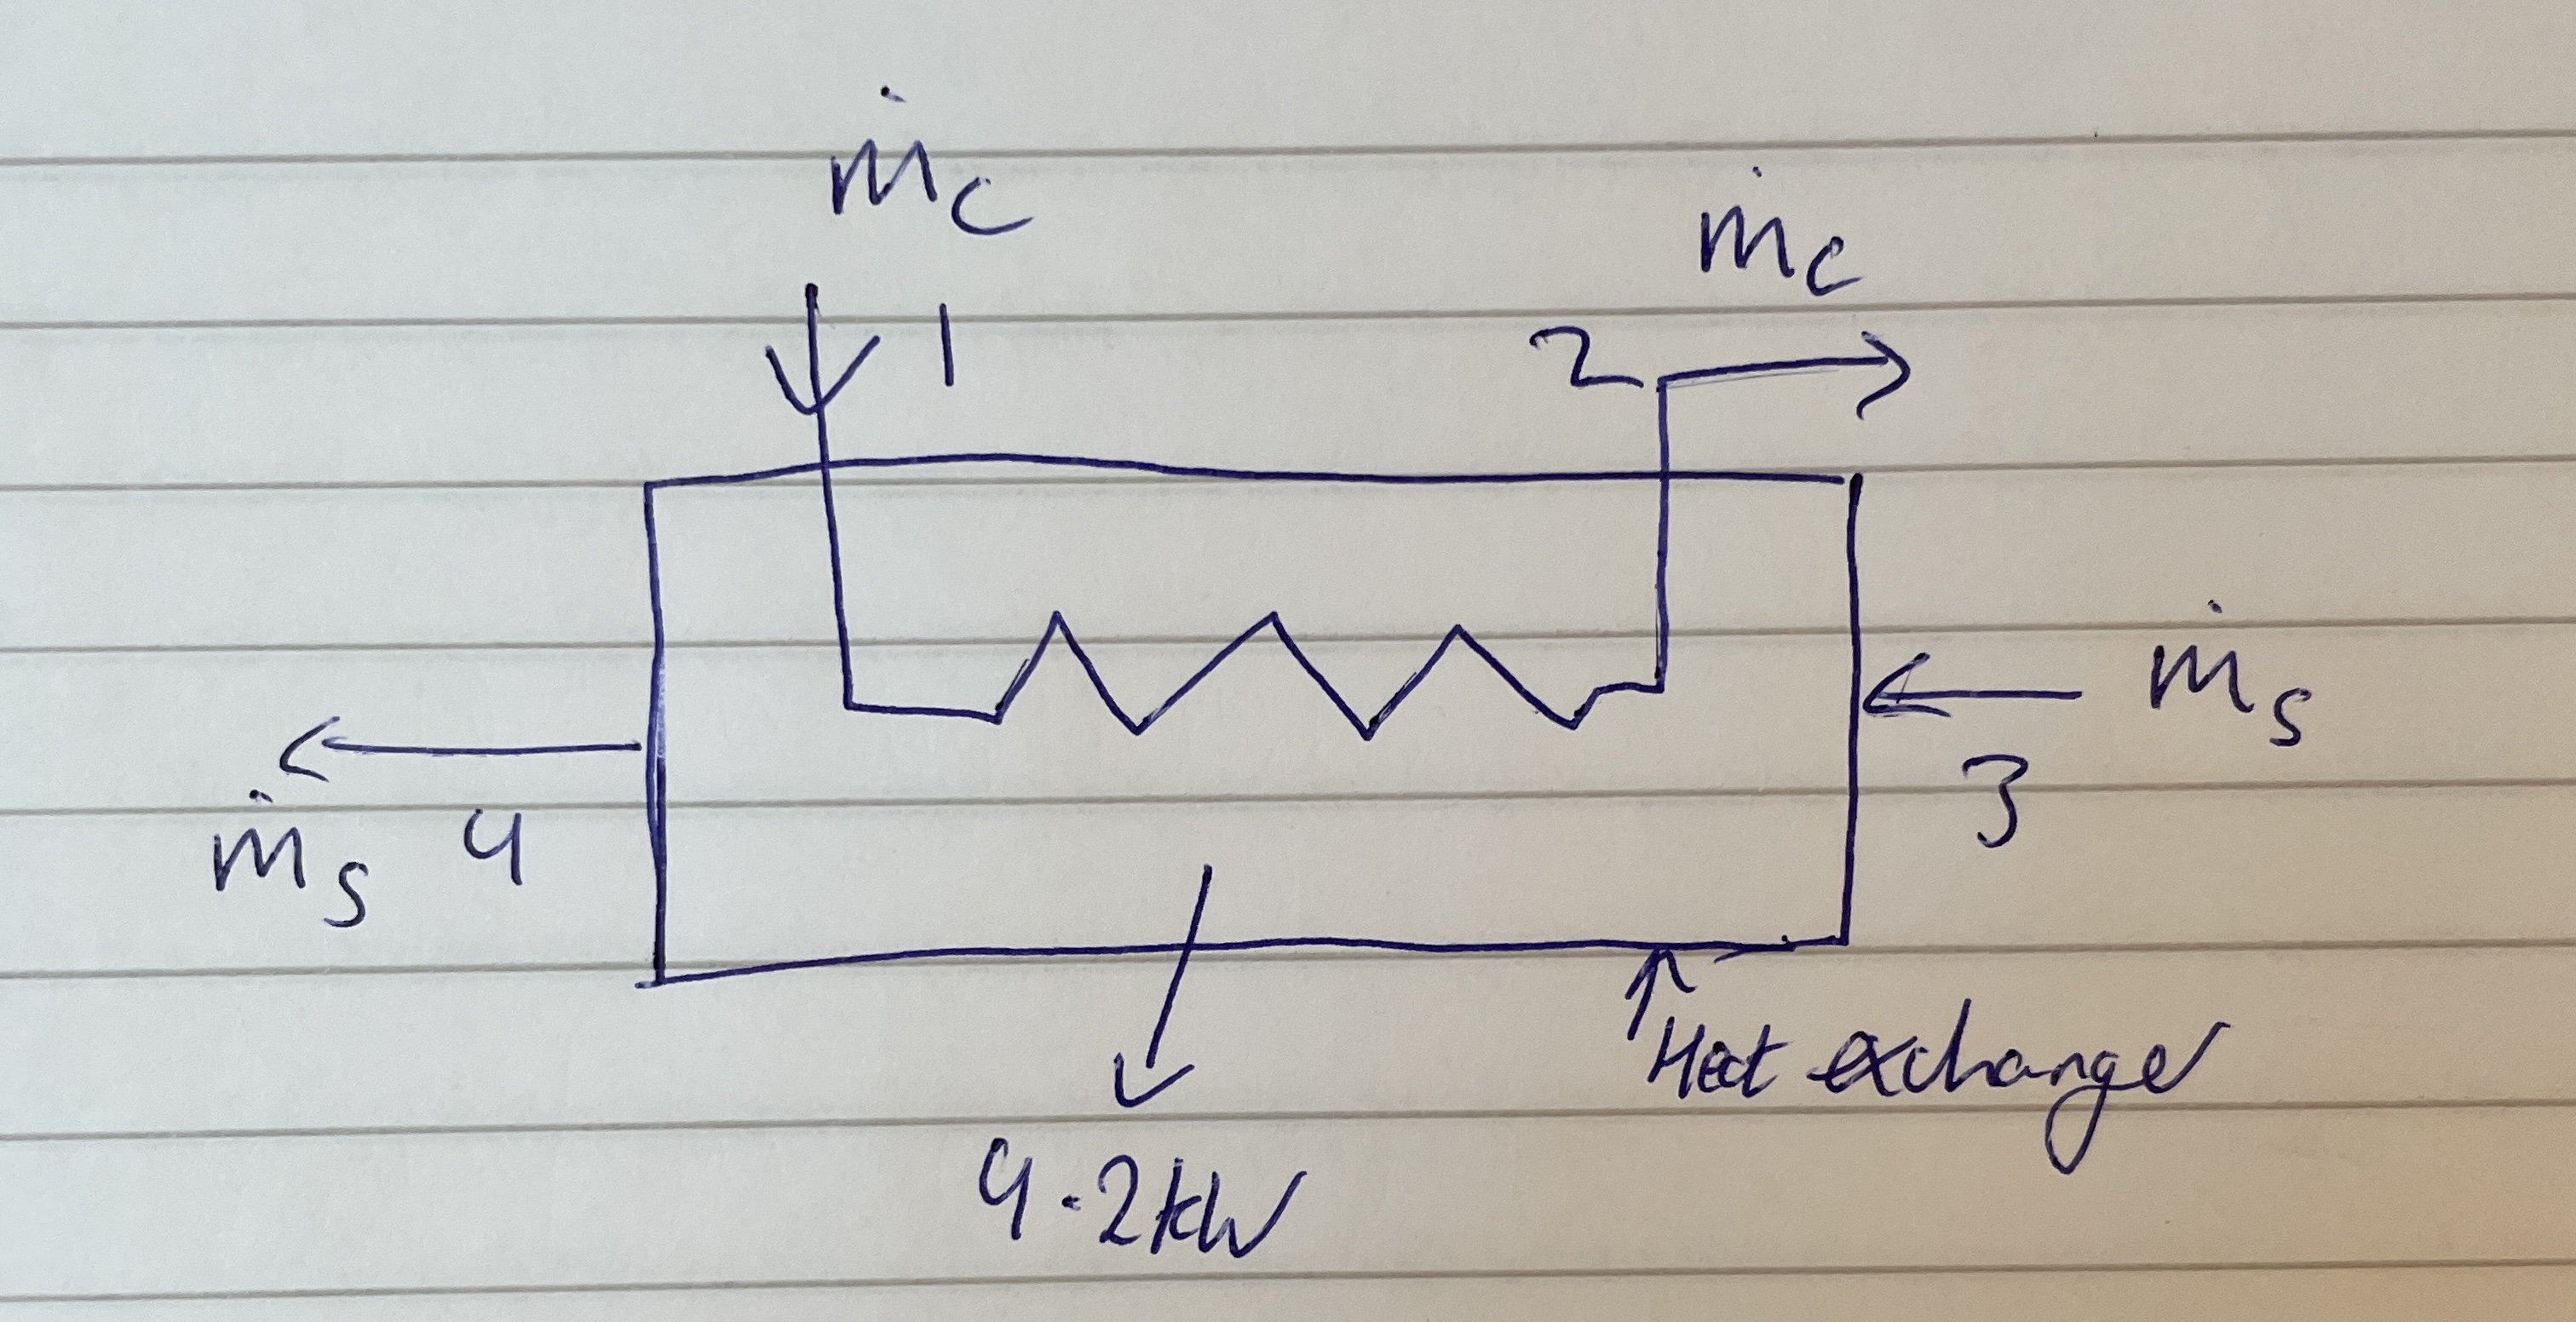
\includegraphics[width = 0.75\textwidth]{img/q2a.JPG}
    \caption{Schematic of heat exchanger.}
\end{figure}
\begin{table}[H]
    \centering
    \begin{tabular}{@{}llllll@{}}
    \toprule
        State & $T$ (\si{\kelvin}) & $P$ (\si{\bar}) & $h$ (\si{\kilo\joule\per\kg})& $s$ (\si{\kilo\joule\per\kg\per\kelvin}) & $\varepsilon = h - T_0 s$ (\si{\kilo\joule\per\kg})\\
        \midrule
        1 & & & & &\multirow{2}{*}{$\varepsilon_1 - \varepsilon_2 = 108$}\\
        2 & & & & &\\
        3 & 506.95 & 30 & 2300.4 & 5.1945 & 751.7\\
        4 & 572.35 & 85 & 2694.6 & 5.6125 & 1011.2\\
        Ambient & 298.15 & 1 & & & \\
        \bottomrule
    \end{tabular}
    \caption{Properties at each state in heat exchanger.}
\end{table}
We know that the irreversibility of the system can be calculated by finding the net loss in exergy:
\begin{align}
    \textrm{net change of exergy} &= \dot{m}_s\left(\varepsilon_3 - \varepsilon_4 \right) + \dot{m}_c \left(\varepsilon_1 - \varepsilon_2\right)\\
    &= 0.23\left(751.7 - 1011.2\right)+ 0.65(108)\\
    &= \SI{10.52}{\kilo\watt}
\end{align}
\subsubsection{Maximum theoretical work available}
\subsection{Relative advantages and disadvantages of four primary energy sources utilised in thermal power generation - chosen: coal, oil, gas, nuclear}
Coal is a low energy density solid which has been used extensively for thermal power generation. It needs to be mined from rocks and transported to plants typically via rail. Coal has limited use cases outside of large-scale power stations since its combustion has limited applications (e.g. cannot be used to make plastics like crude oil). Coal’s use can also be problematic since it is a greenhouse gas and often suffers from contamination such as sulphur, which presents an environmental problem when combusted. Coal is largely being phased out in the UK in favour of alternatives. 

Oil and gas can be pumped from reserves underground and can be transported in barrels or tanks. Since oil is a high energy density liquid, this makes it cheaper to use. However, crude oil requires fractionation to separate it into usable chemicals (a few of which can be used for thermal power generation). Natural gas is relatively low energy density but requires no additional processing for use. Oil and gas are both hydrocarbon based, hence the aforementioned greenhouse gases emitted during combustion present a climate risk. Oil and gas reserves are running out; hence these are also being phased out in favour of alternatives and climate awareness.

Nuclear power has seen recent resurgence as it has been touted as a cleaner alternative to fossil fuels. It has low carbon emissions and unknown and potentially very long-lasting reserves. However, there have been issues with safety with some catastrophes such as Chernobyl and Fukushima. Nuclear power also requires highly skilled workers to construct and operate making them unavailable to poorly developed/developing countries. Since uranium deposits are only in a select few countries, it must be imported for many countries, presenting additional cost for countries looking to invest. Nuclear power also generates highly dangerous waste which takes millennia to dispose of. This may be mitigated with the development of new reactor types. Nuclear power has the potential to replace current fossil fuel plants given enough investment and research into the area.
\section{Question 3}
\subsection{a}
\subsubsection{Mass of methane present}
\subsubsection{Approximate level of \ce{CO} in exhaust gases}
\subsection{Effects of fuel molecular composition on ignition, temperatures and formation of exhaust pollutants during combustion}
Hydrocarbon based fuels will produce some pollutants when combusted. This can be due to a variety of reasons such as incomplete combustion producing carbon monoxide and leaving unburnt hydrocarbons in the exhaust. Dissociation of exhaust products will also form nitrous oxides and other species. We may also see some contamination in the form of particulate matter and sulphur oxides. Due to the low reaction times in combustion engines, these reactions cannot reach equilibrium and are rate-controlled, hence the formation of these unwanted molecules. On fuel ignition under stoichiometric conditions, the hydrocarbon fuel will break down to form water and carbon dioxide, alongside other molecules. This produces greenhouse gases, which contribute to climate change. Some engines run lean which increases formation of \ce{NO_x}. \ce{NO_x} production greatly increases with temperature. On the other hand, rich fuel ratios produce higher amounts of \ce{CO} and \ce{H_2}. The formation of these molecules inherently represents an inefficiency in combustion, but the reduction of their formation has a limit due to the operating conditions of an engine. 

Renewable fuels must be developed to avoid the formation of unwanted molecules. Currently, Euro 6 emissions regulations cannot be met solely by optimising combustion within the engine, requiring exhaust catalysts and filters, which add cost to the vehicle. Hence, renewable fuels must be designed to be easily sourced whilst producing minimal particulate matter and/or damaging products. The reduction of particulate matter and \ce{NO_x} can be achieved by reducing the contaminants within the fuel and optimising AFR and combustion timing within the cycle. However, unless there is a change in the way engines are designed, renewable fuels will suffer from the same underlying issues. 

A better solution may be to offload the combustion cycle to larger power plants, where combustion can be highly optimised outside of a rate-controlled reaction and the subsequent energy used to charge battery electric vehicles. The renewable fuels used can hence be designed specifically for use in larger boilers heating steam. Lower temperatures may be permissible and equilibrium conditions are easily reachable as the combustion has time to occur fully.  

\section{Question 4}
\subsection{a}
\subsubsection{Ideal operating voltage}
Applying steady flow energy equation
\begin{gather}
    \dot{Q} - \dot{W} = \dot{m}\left(h_{P0} - h_{R0}\right)
\end{gather}
where $\dot{Q}$ is our heat loss, $\dot{W}$ is our work done, $\dot{m}$ is the mass flow rate, $h_{P0}$ is enthalpy of products and $h_{R0}$ is enthalpy of reactants. 

Since we are considering an ideal fuel cell, we can utilise the following:
\begin{gather}
    \dot{Q} = \dot{m}T_0\left(s_{P0} - s_{R0}\right)
\end{gather}
Therefore:
\begin{gather}
    \dot{W} = \dot{m}T_0 \left(s_{P0} - s_{R0}\right) - \dot{m}\left(h_{P0}-h_{R0}\right)\\
    \dot{W} = \dot{m}\left[\left(h_{R0} - T_0s_{R0}\right)-\left(h_{P0}-T_0s_{P0}\right)\right]
\end{gather}
We know that:
\begin{gather}
    \textrm{Gibbs function} = h- Ts
\end{gather}
Therefore:
\begin{gather}
    \dot{W} = -\dot{m}\Delta G  
\end{gather}
In this case:
\begin{gather}
    45 = - \dot{m} \left(-226500\right)\\
    \dot{m} = \frac{45}{226500} = \SI{1.99e-04}{\kilo\mol\per\second}
\end{gather}
We also know:
\begin{gather}
    \dot{W} = V\mathcal{F}n\dot{m}
\end{gather}
where $V$ is the ideal operating voltage, $\mathcal{F}$ is Faraday's constant and $n$ is number of charge transfers per molecule of fuel. Hence:
\begin{gather}
    V = \dfrac{\dot{W}}{\mathcal{F}n\dot{m}}\\
    V = \dfrac{45\cdot 226500}{96485\cdot 2 \cdot 45} = \SI{1.1738}{\volt}
\end{gather}
\subsubsection{Anode area}
We know that:
\begin{gather}
    P = IV\\
    I = \dfrac{45000}{1.1738} = \SI{38338}{\ampere}
\end{gather}
Therefore, the anode area necessary is:
\begin{gather}
    \textrm{Anode area} = \dfrac{38338}{6500} = \SI{5.8982}{\meter\squared}
\end{gather}
\subsubsection{Heat loss}
Applying steady flow energy equation (subscript a denotes `actual'):
\begin{gather}
    \dot{Q}_a - \dot{W}_a = \dot{m}\Delta H\\
    \dot{Q}_a = \dot{m}\Delta H + 2 \cdot \dot{m} \mathcal{F}V_{a}\\
    \dot{Q}_a = \frac{45}{226500}\left(-239800\cdot 10^3 + 2\cdot 96.485\cdot 10^6 \cdot 0.984\right)\\
    \dot{Q} = \SI{-9.92}{\kilo\watt}
\end{gather}
\subsection{Limitations of hydrogen oxygen fuel cell vehicles}
Fuel cell vehicles have been designed and manufactured since the 60s, due to the use of alkaline fuel cells by NASA. Nowadays, we see that fuel cell vehicles are not popular, rather internal combustion engine, hybrid and battery electric cars take up the vast majority of vehicle market share. Currently, there are only two publicly available fuel cell vehicles, both of which use solid-polymer fuel cells \cite{b3} \cite{b4}. Solid-polymer cells have a high-power density and an operating temperature low enough to not be hazardous. This low operating temperature also allows the cell to start quickly. However, these cells have low efficiencies, limiting their effectiveness. Solid-polymer cells suffer from a variety of losses such as activation losses, fuel crossover/internal current losses, ohmic losses and mass transport losses. These are mitigated by fuel cells utilising different technologies such as solid oxide or molten carbonate, however these cells must operate at very high temperatures making them unsuitable for use in cars.

Due to their small and niche market size, there is little support for such vehicles in today's world. In the UK, there are only 17 hydrogen filling stations making their convenience low. ICE cars have been sold for over 120 years and thus the infrastructure developed around them is extensive. Alternative renewable fuels are a much better interim solution as they can be integrated directly into current infrastructure. Recently there has been a large shift towards battery electric vehicles, with extensive charging networks being developed and investment from all major vehicle manufacturers. Battery electric vehicles can be charged at home and are less complex from an engineering perspective than fuel cell vehicles. Fuel cell vehicles require high-pressure hydrogen tanks and expensive catalysts in the cell itself, presenting a safety and cost issue for manufacturers. This also makes them harder to service and maintain as typically trained technicians need to fix these vehicles. To the end user, fuel cell vehicles are an expensive and inconvenient way to reduce their carbon footprint, whereas using renewable biofuels or driving electric vehicles are an easier way of doing so. Biofuel is currently available at most petrol stations and there are a large range of electric vehicles on sale today.

\newpage
\begin{thebibliography}{00}
    \bibitem{b1} Week 1 Lecture Slides Thermodynamics, Dr Paul Hellier, MECH0024 Advanced Thermodynamics and Fluid Mechanics, \url{https://moodle.ucl.ac.uk/pluginfile.php/3766587/mod_resource/content/1/MECH0024%20Thermodynamics%20-%20Topic%201%20Global%20energy%20supply.pdf} [Last accessed 27/03/22]
    \bibitem{b2} UCL Live Energy data, SustainableUCL, \url{https://www.ucl.ac.uk/sustainable/staff/positive-climate-resources/energy-saving-resources/ucls-live-energy-data#:~:text=Each%20year%2C%20powering%2C%20lighting%2C,%C2%A316%20million%20in%20energy} [Last accessed 27/03/22]
    \bibitem{b3} Toyota Mirai Hydrogen Fuel Cell Vehicle, `New Mirai hydrogen fuel cell electric vehicle - under the skin', article by Matt Burt, \url{https://mag.toyota.co.uk/new-mirai-hydrogen-fuel-cell-electric-vehicle/ } [Last accessed 27/03/22]
    \bibitem{b4} Hyundai Nexo, article by Drew Dorian, \url{https://www.caranddriver.com/hyundai/nexo} [Last accessed 27/03/22]
\end{thebibliography}
\end{document}